\documentclass[letterpaper,draft]{article}

%pass the page height/width into pdflatex, otherwise it assumes A4
\pdfpagewidth=\paperwidth
\pdfpageheight=\paperheight

\usepackage{graphicx} %get graphics commands
\usepackage{times}

%get \FloatBarrier command
\usepackage{placeins} 

%give option to use commands like 0.5\textwidth for distances
\usepackage{calc} 
 %allows wraping figures around text
\usepackage{wrapfig}

%adds option to include verbatim input from files
\usepackage{moreverb} 

%Set the pages margins to 1 inch, all the way around
\usepackage{anysize}
\marginsize{1in}{1in}{0.45in}{0.45in}

\usepackage{setspace}
%\doublespace

\begin{document}

\begin{figure}[htbp]
\begin{center}
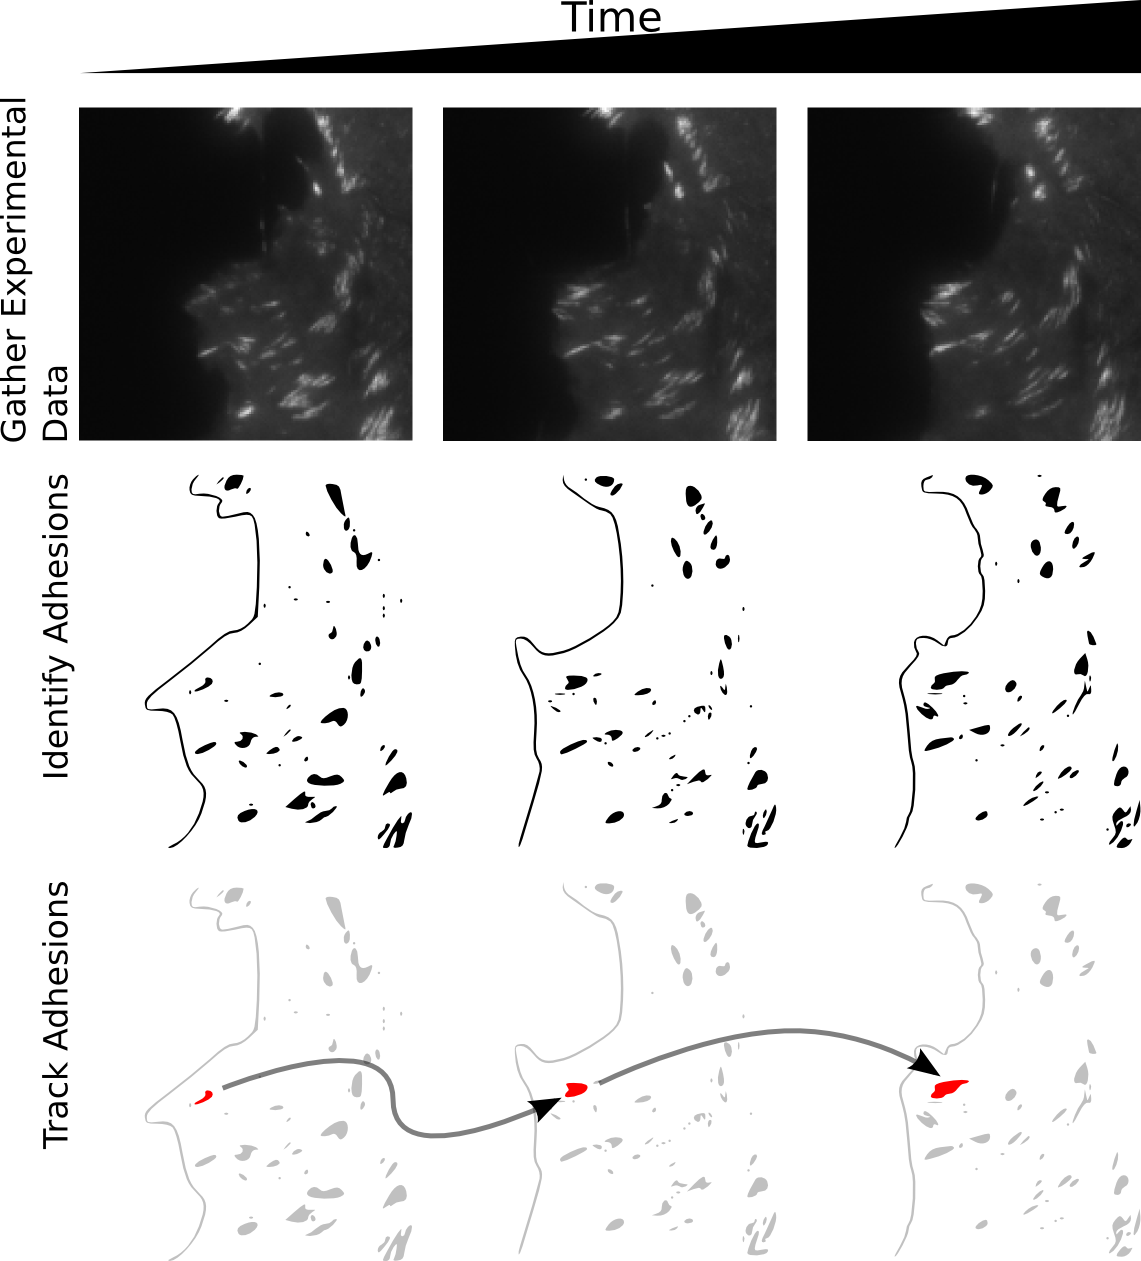
\includegraphics[width=\textwidth]{../figures/FA_workflow/graphic_workflow}
\caption{
{\bf Automating the analysis of focal adhesion images requires a multi-stage pipeline.} First, high-resolution time-lapse TIRF fluorescent microscopy images of a focal adhesion component are collected. The example images are of EGFP-paxillin in NIH 3T3 cells. Second, the adhesions are segmented, producing data sets of static adhesions. Third, the adhesions are tracked through the experiment, making it possible to collect data about the dynamic properties of the adhesions. The bar is 10 $\mu$m.
}
\label{method_flow}
\end{center}
\end{figure}

\begin{figure}[htbp]
\begin{center}
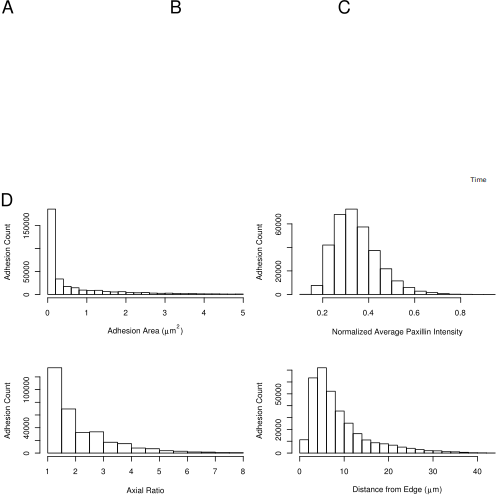
\includegraphics[width=\textwidth]{../figures/statics/statics}
\caption{
{\bf Applying quantitative image processing methods to FA images allows comprehensive characterization of FA properties.} (A) One frame from a 200 minute movie of NIH 3T3 cells expressing GFP-Paxillin (the scale bar represents 10$\mu$m). (B) The same cell as in (A), with each adhesion outlined in a different color. (C) The entire set of adhesions in an experiment can be visualized by overlaying the adhesions from each microscopy image going from the first image collected to the last image collected. (D) A large range of properties can be extracted from the segmented FA, distributions for three properties are shown.
}
\label{statics}
\end{center}
\end{figure}


\begin{figure}[htbp]
\begin{center}
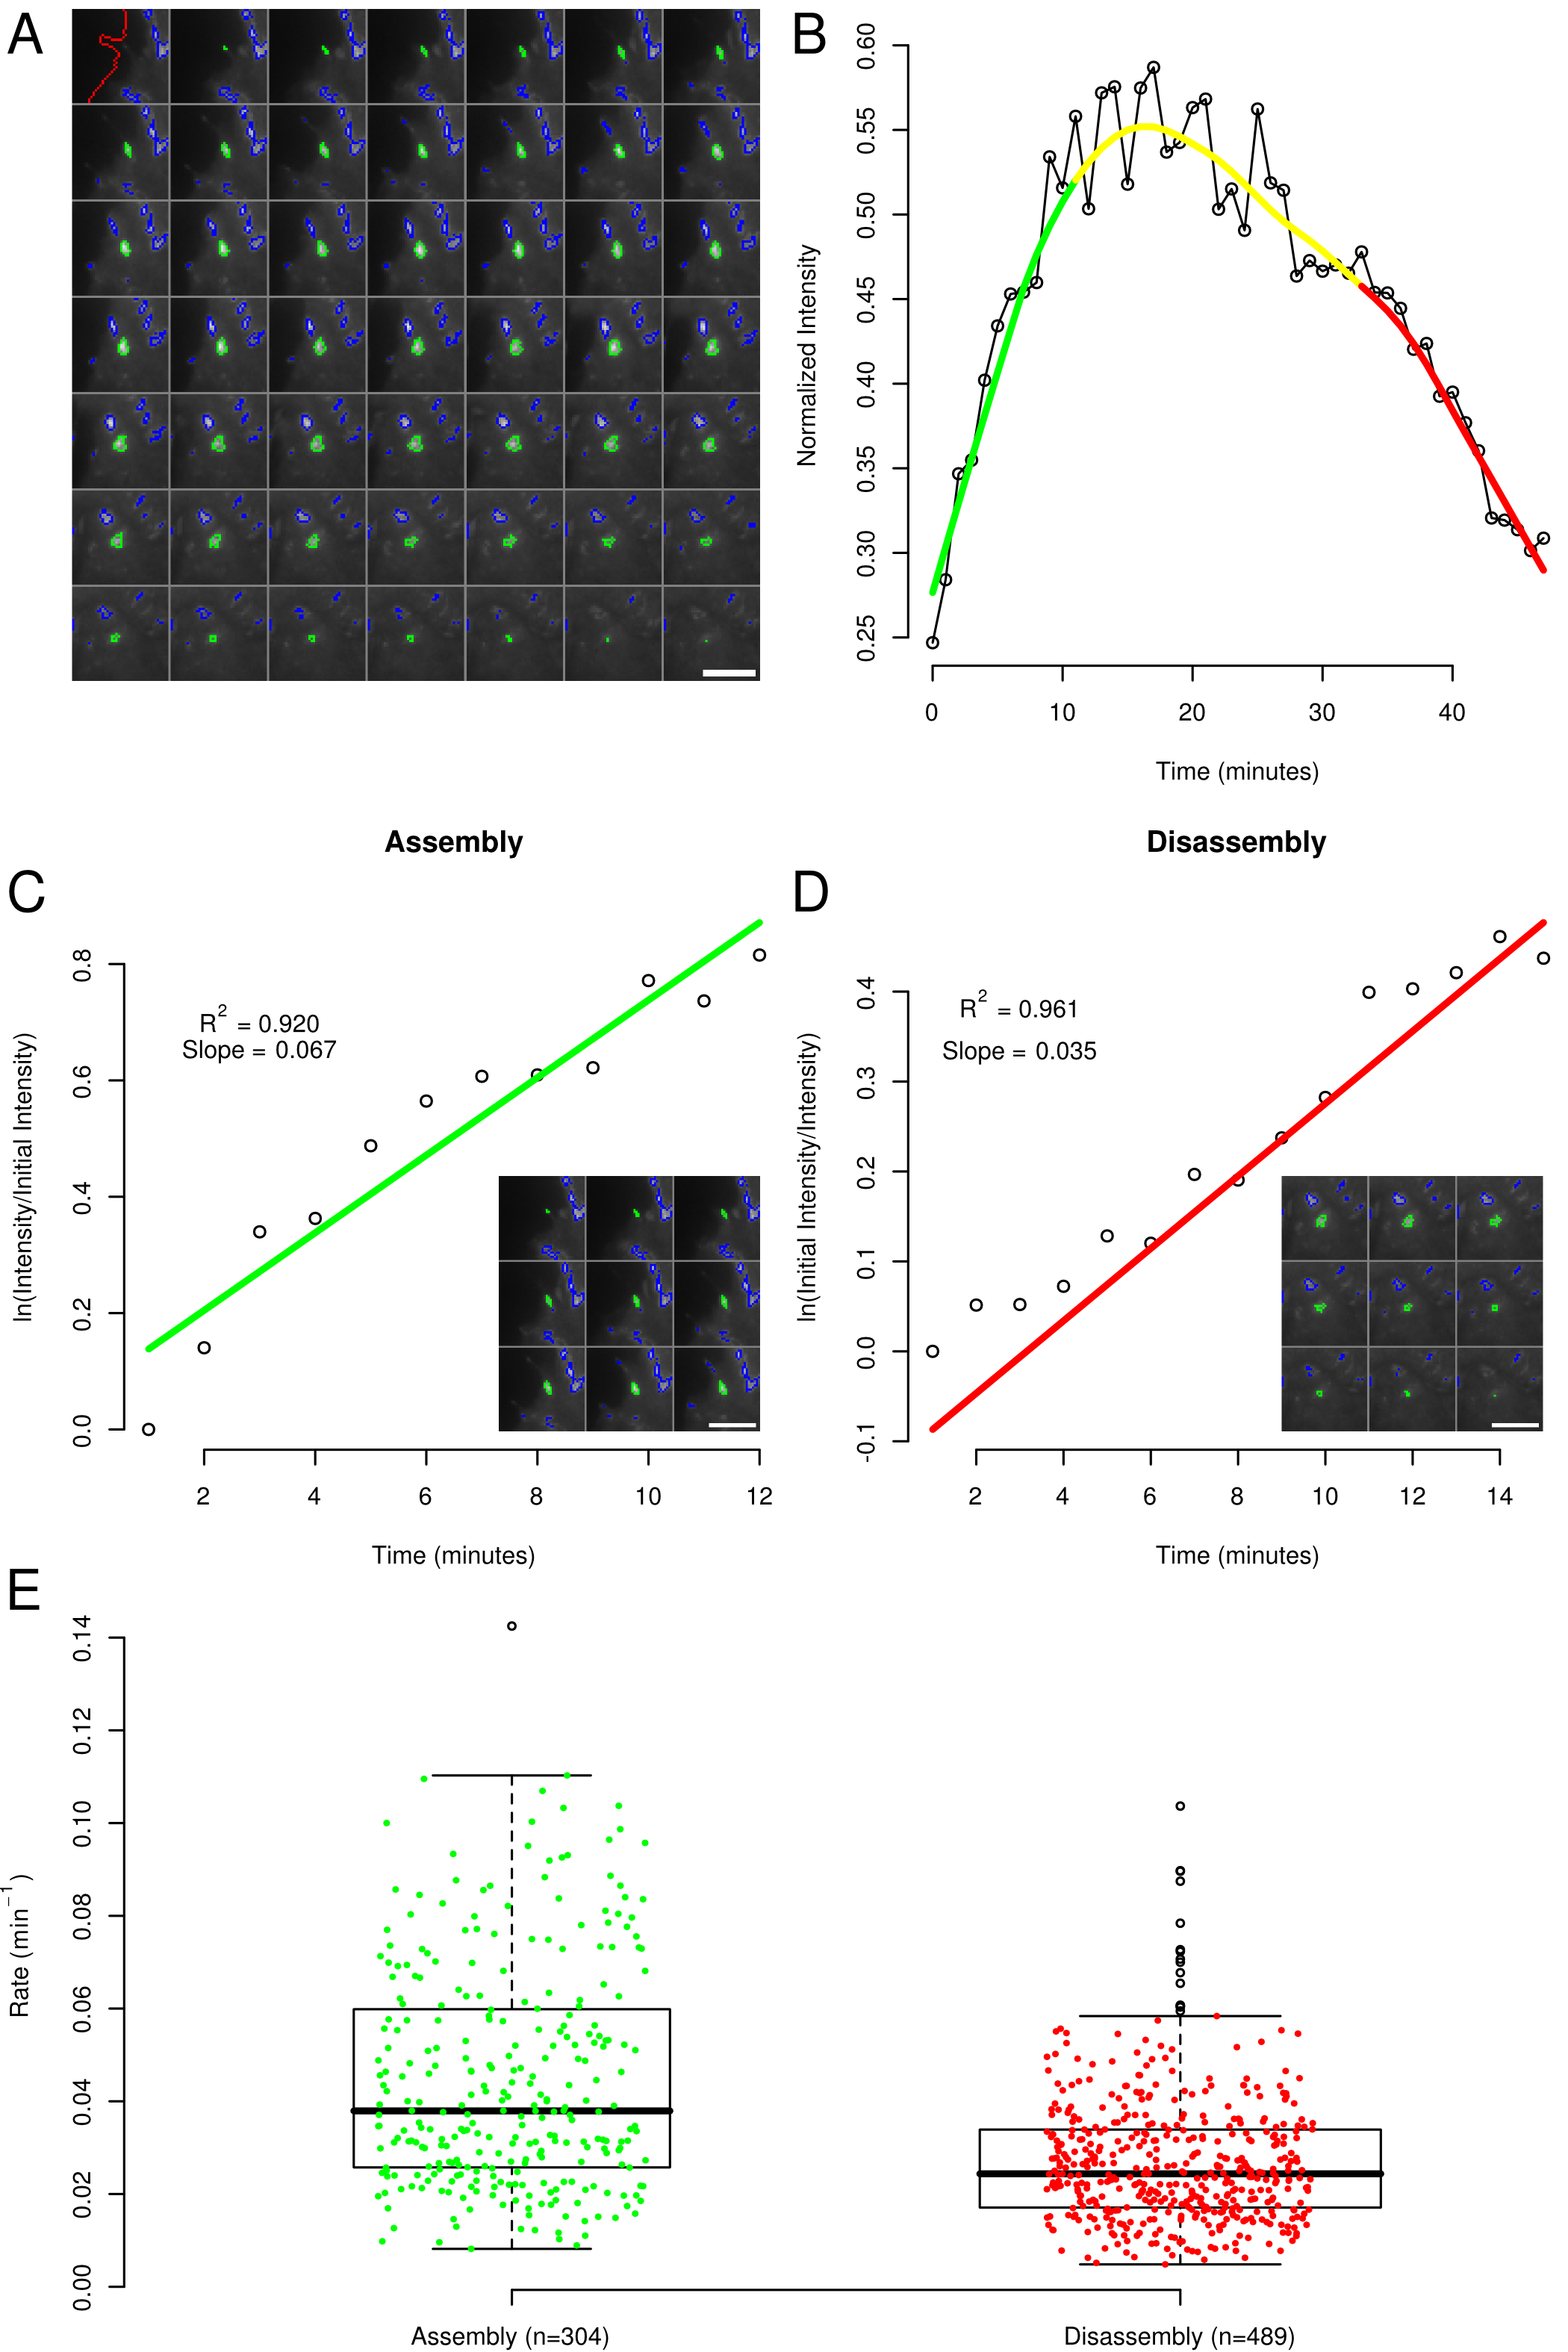
\includegraphics[height=0.8\textheight]{../figures/kinetics/kinetics}
\caption{
{\bf Focal adhesion kinetics.} (A) Each of the adhesions in the cells is tracked, allowing the position and properties of single adhesions to be assessed. Here a single adhesion (in green), the surrounding adhesions (in blue) and the cell edge (in red) are followed for 49 minutes. The cell edge is only outlined in the first frame. (B) The intensity of the paxillin in the tracked adhesion in (A) through time. The red line is a smoothed fit to the data using the lowess algorithm. (C) The normalized log-linear fit of the Paxillin intensity through time during the assembly phase of the adhesion in part (B). The inset depicts several of the images from which the Paxillin intensity was gathered. The color highlights indicate the same cell features as in (A). (D) The normalized log-linear fit of the Paxillin intensity through time during the disassembly phase of the adhesion in part (B). The inset depicts several of the images from which the Paxillin intensity was gathered. The color highlights indicate the same cell features as in (A). (E) The assembly and disassembly rates for adhesions whose Paxillin intensity curve fits have R$^2$ values of 0.9 or greater. The scale bar is 10 $\mu$m.
}
\label{kinetics}
\end{center}
\end{figure}

\begin{figure}[htbp]
\begin{center}
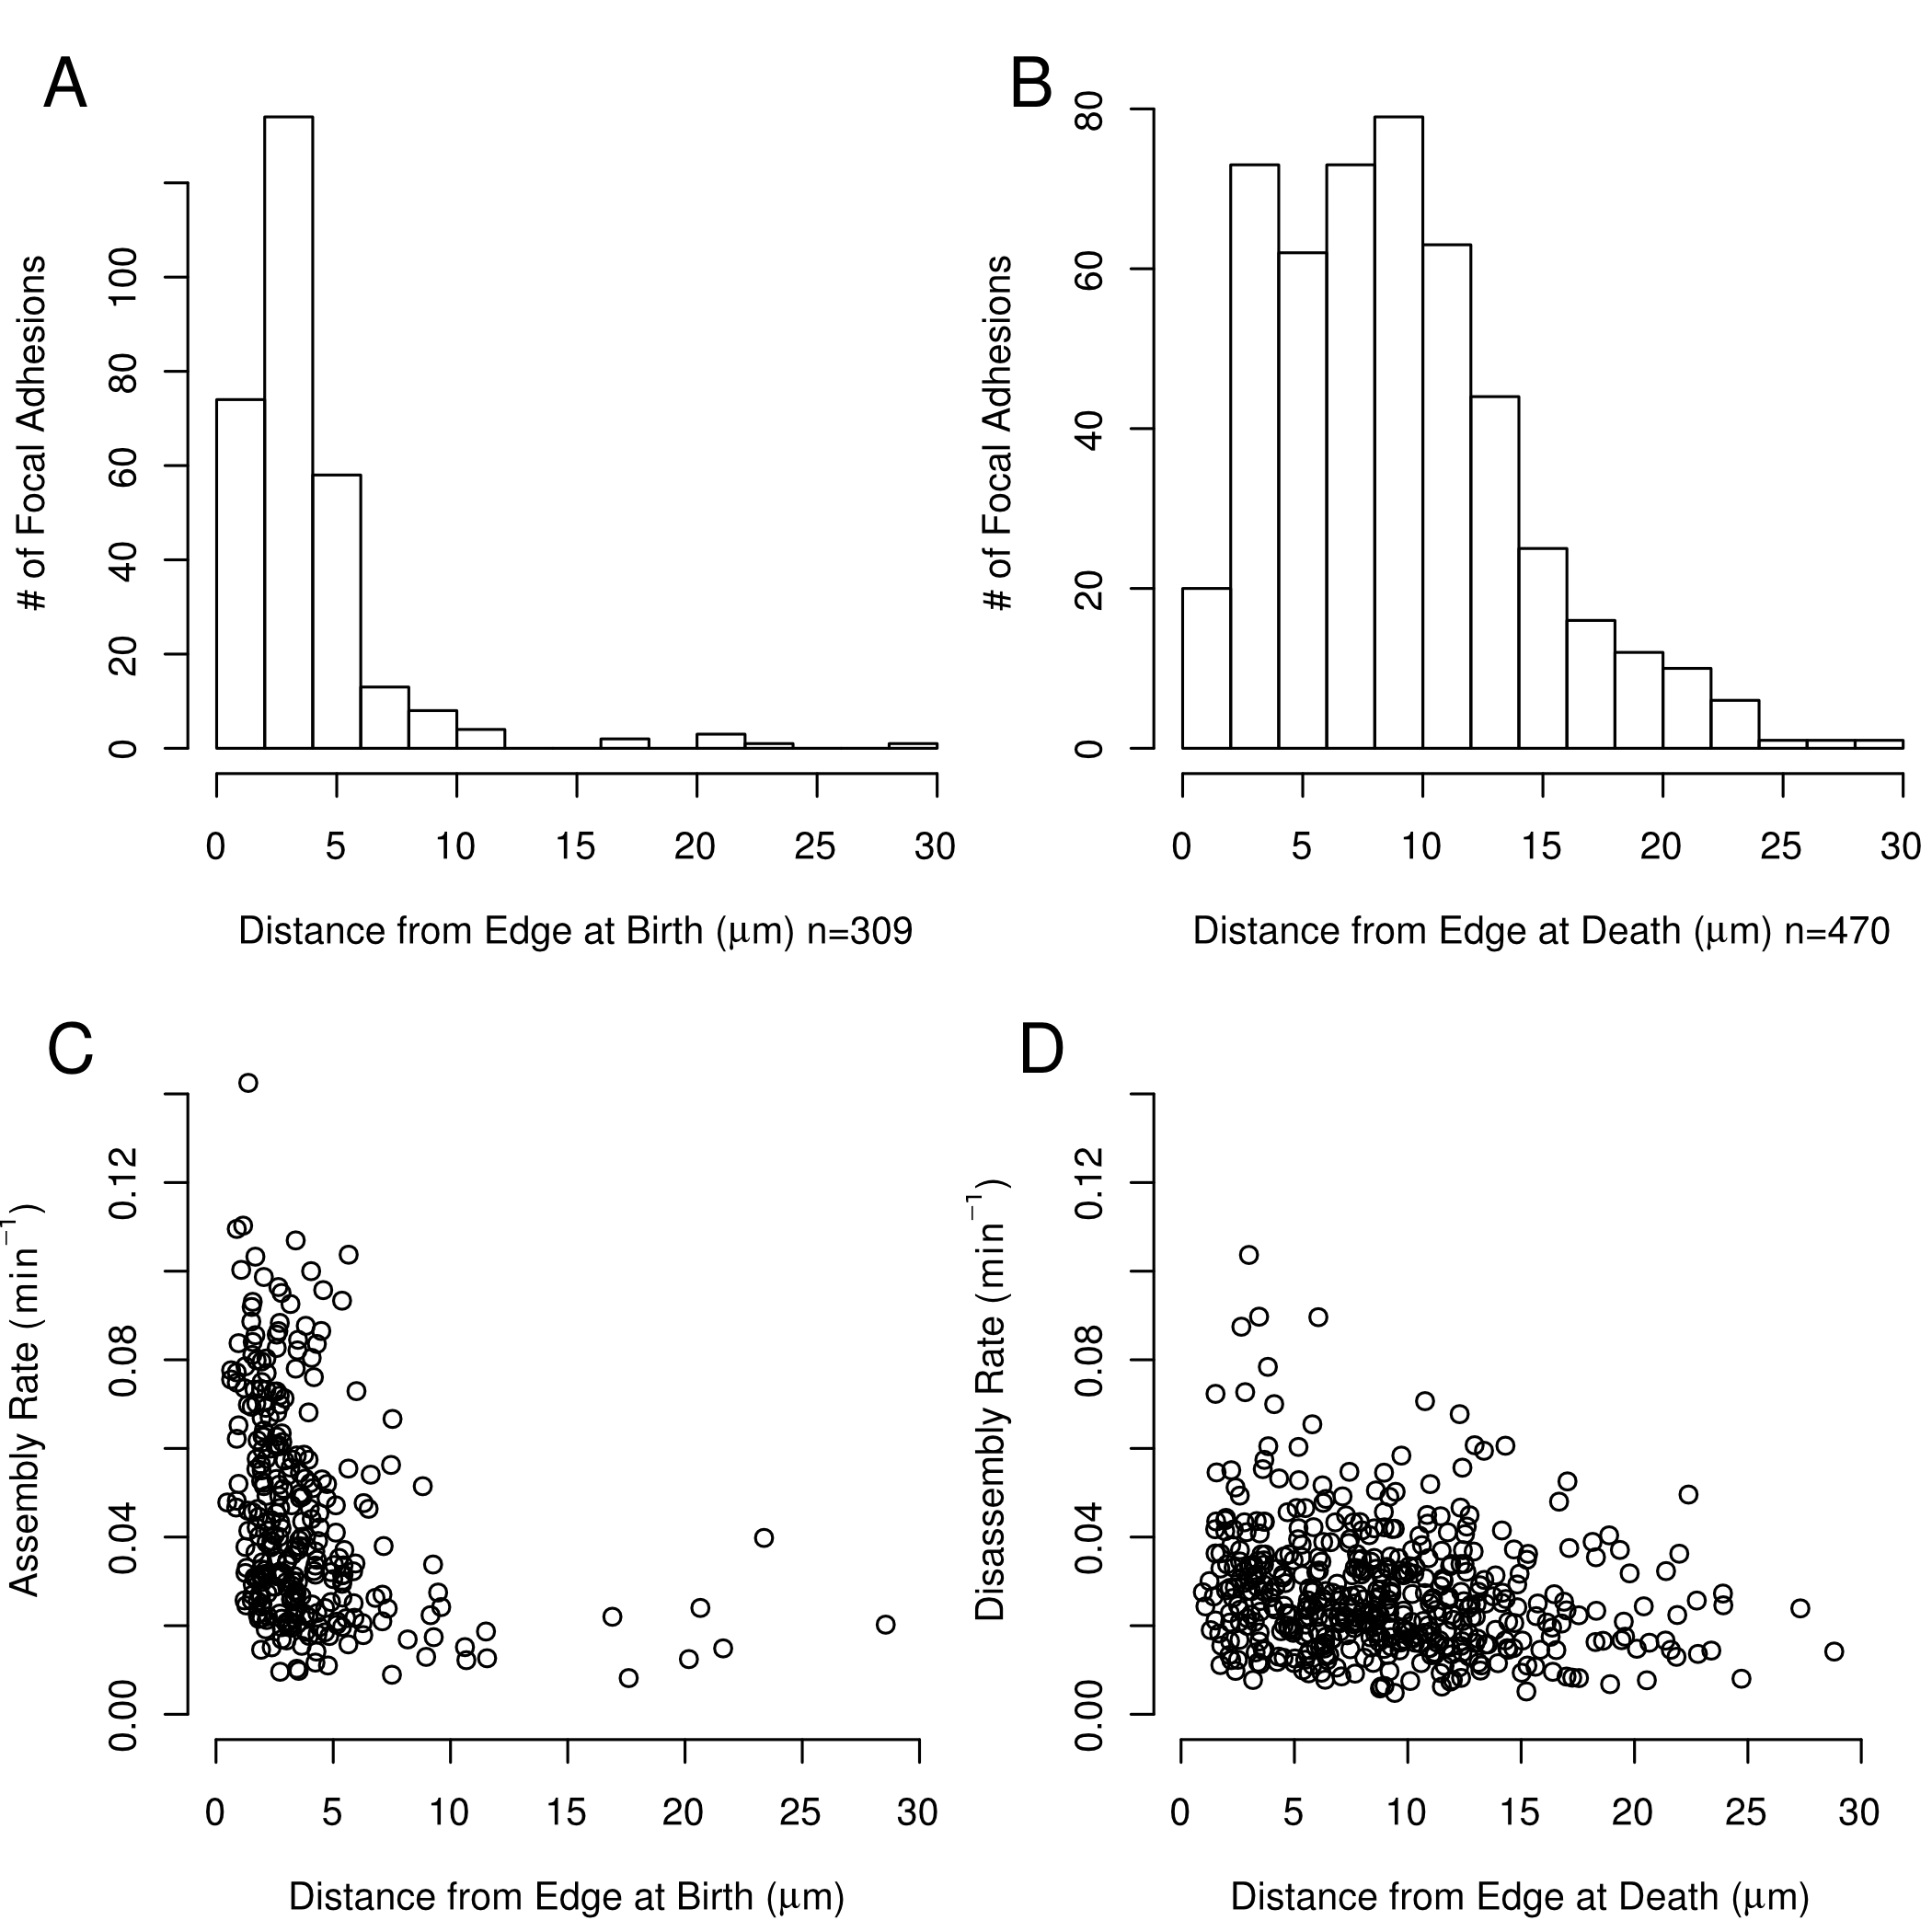
\includegraphics[width=\textwidth]{../figures/spacial/spacial}
\caption{
{\bf Spacial properties of FA centroid positions at birth and death where the assembly and/or disassembly phases fit a log-linear model with R$^2$ value of 0.9 or greater.} (A) The majority of adhesions whose growth patterns demonstrate a strong linear model are born within 5 $\mu$m of the cell edge. (B) The distribution of the distance of death location from the cell edge indicates that adhesion disassembly typically occurs along a broader band at the cell edge as compared to the position at adhesion birth. (C) The variance of assembly rates is greatest for adhesions born within $\sim$5$\mu$m of the edge (D) The variance of disassembly rates only has a slight decrease as the distance from edge at death increases.
}
\label{spacial}
\end{center}
\end{figure}

\begin{figure}[htbp]
\begin{center}
\includegraphics[width=\textwidth]{../figures/lifetimes/adhesion_phase_lifetimes}
\caption{
{\bf The assembly phases in S178A mutant FA are significantly longer than those in the wild-type, while the stability and disassembly phase lengths are unaffected.} Error bars indicate 95\% confidence intervals on the mean as determined through bootstrap 50,000 bootstrap samples. A single asterisk (*) indicates $p<0.01$ (bootstrap confidence interval).
}
\label{lifetimes}
\end{center}
\end{figure}


\begin{figure}[htbp]
\begin{center}
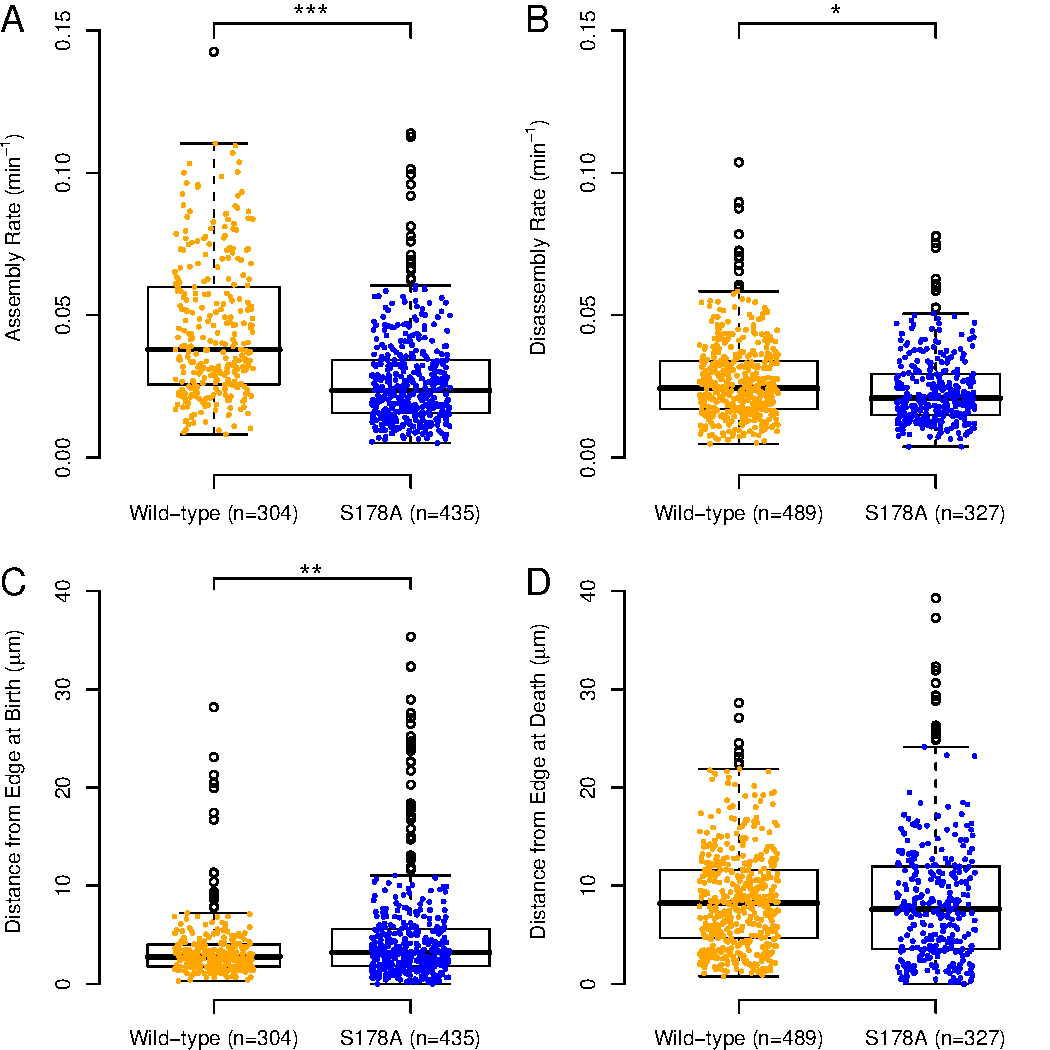
\includegraphics[width=\textwidth]{../figures/S178A/S178A_vs_wild-type}
\caption{
{\bf Comparison between several of the properties of the S178A mutants and wild-type FA in adhesions which fit a log linear model with R$^2$ value of 0.9 or greater.} (A) The mean assembly rate is decreased by 40\% in the S178A case ($p<10^{-5}$). (B) The mean disassembly rate is also decreased, but only by 16\% ($p<10^{-3}$). (C and D) The median position of adhesion centroids at birth is increased by 44\% ($p<10^{-3}$), while the median position of the adhesion centroid at death is unaffected in the S178A mutants. All p-values were calculated using the bootstrapped confidence intervals.
}
\label{S178A}
\end{center}
\end{figure}

\end{document}